\section{rSLA runtime engine}\label{runtime}

The rSLA is implemented as a DSL for cloud SLAs. The rSLA programming library, currently, provides support for the following SLA management operations that take place while a provisioned service is running:
\begin{enumerate}
\item SLA creation and activation.
\item monitoring and measurement of service metrics as specified by the SLA context.
\item storage and processing of observed service metric values and of SLO evaluation results. 
\item scheduling of rSLA objects.
\item service level evaluation.
\item notification events: reports.
\end{enumerate}
The next paragraphs highlight rSLA implementation aspects for all supported operations.

\subsection{SLA creation and activation}

As discussed in Chapter \ref{dsl}, rSLA editing takes place using ruby programming blocks. The rSLA language takes advantage of this Ruby coding feature and exposes rSLA objects through multi-lined do..end coding blocks. When an rSLA runtime engine reads a new rSLA block, it generates a new rSLA object that belongs to the block related class. The attributes and function behavior of the generated object are mapped from the ruby block context. 

Listing \ref{basescript} describes an rSLA script for the creation of an SLA and of a base metric. The script can run in an rSLA service runtime environment to generate the two respective objects and to activate a schedule for the value measurement of the base metric.

\begin{minipage}{0.9\textwidth}
\begin{lstlisting}[language=Ruby, basicstyle=\small\normalfont\sffamily, breaklines=true,  captionpos=b, mathescape=true, caption=rSLA SLA (lines 1-4) and basemetric (lines 6-19) creation script, label=basescript, numbers=left, numbersep=5pt, numberstyle=\tiny] 
sla do
  tenant "Demo"
  provider "IBM"
end  

basemetric do
    name "bareMetalProvisioning"
    unit "provisioningtime"
    measurementdirective do
    	entity "baremetal"
    	type "jsonArray"
    	source "http://provisioningxlet.stage1.mybluemix.net/server/baremetal/provisioningtime" 
  	end
  schedule do    
  	frequency "1"
    unit "m"
    method "every"
  end
end
\end{lstlisting}
\end{minipage} 

The block for the creation of the SLA object simply describes two strings that designate the names of the SLA tenant and provider. The rSLA engine reads such strings as the attribute values of the newly created SLA object. Similarly, the rSLA interpreter reads the base metric block and create a new base metric object that inherits the attributes of the rSLA BaseMetric class. 

In the base metric block, a DSL user can define BaseMetric object attributes like the base metric name and measurement unit. Additionally, a DSL user can specify directives for the measurement of the created metric. A measurement directive represents a concept that is inherited from the WSLA specification \cite{wsla}. 

The rSLA DSL exposes a measurement directive as a block of statements that a DSL user can specify. Such statements describe the configuration of a measurement directive object that guides the value measurement of the parent base metric. A measurement directive indicates the result type that is expected from a base metric measurement.

In the measurement directive block, the term entity is used for the representation of restful \footnote{ReST: \url{http://en.wikipedia.org/wiki/Representational_state_transfer}} endpoints. Such may have a URL\footnote{Unique Resource Locator: \url{http://en.wikipedia.org/wiki/Uniform_resource_locator}} form: \url{http://provisioningxlet.stage1.mybluemix.net/server/baremetal/provisioningtime}. A measurement directive object uses an attribute named $source$ to denote the restful endpoint for fetching the relevant base metric value. The rSLA MeasurementDirective class provides an example on how to define measurement directive objects for rSLA base metrics. Such example, like the illustrated block of Listing \ref{basescript} can be extended accordingly. 

Last but not least, a DSL user can specify the details of a schedule for the measurement of the base metric. The schedule block details are explained in Section \ref{schedule}.

\subsection{monitoring and measurement}
Any SLA management framework for cloud services needs a tool for monitoring and measuring service metric values. In a cloud runtime environment, an rSLA service currently uses Java Xlets \cite{xlets} to handle the monitoring of base betric values. Chapter \ref{deployment} describes in detail the configuration and functionality of Xlets with the deployment of rSLA as a compliance service in a cloud environment.

In an rSLA service, monitoring and measurement operations are controlled by one or more schedules. Every base metric follows its own schedule. Measured metric values are collected to a backend database for further processing. 
\subsection{storage and processing}
Observed values of base metrics are stored during service provisioning. These data values are required for the computation of composite metric values, which in turn are used in the service level evaluation. 

Currently, rSLA has been deployed using the Cloudant document database \cite{cloudant}. The values of base metrics are preserved as observation documents that also keep a timestamp on the measurement time and the associated base metric id. Cloudant uses map and reduce statements to collect and to efficiently process data values. 

Associations between rSLA objects are, at the present time, described through the rSLA data schema in cloudant.

\begin{figure}
\centering
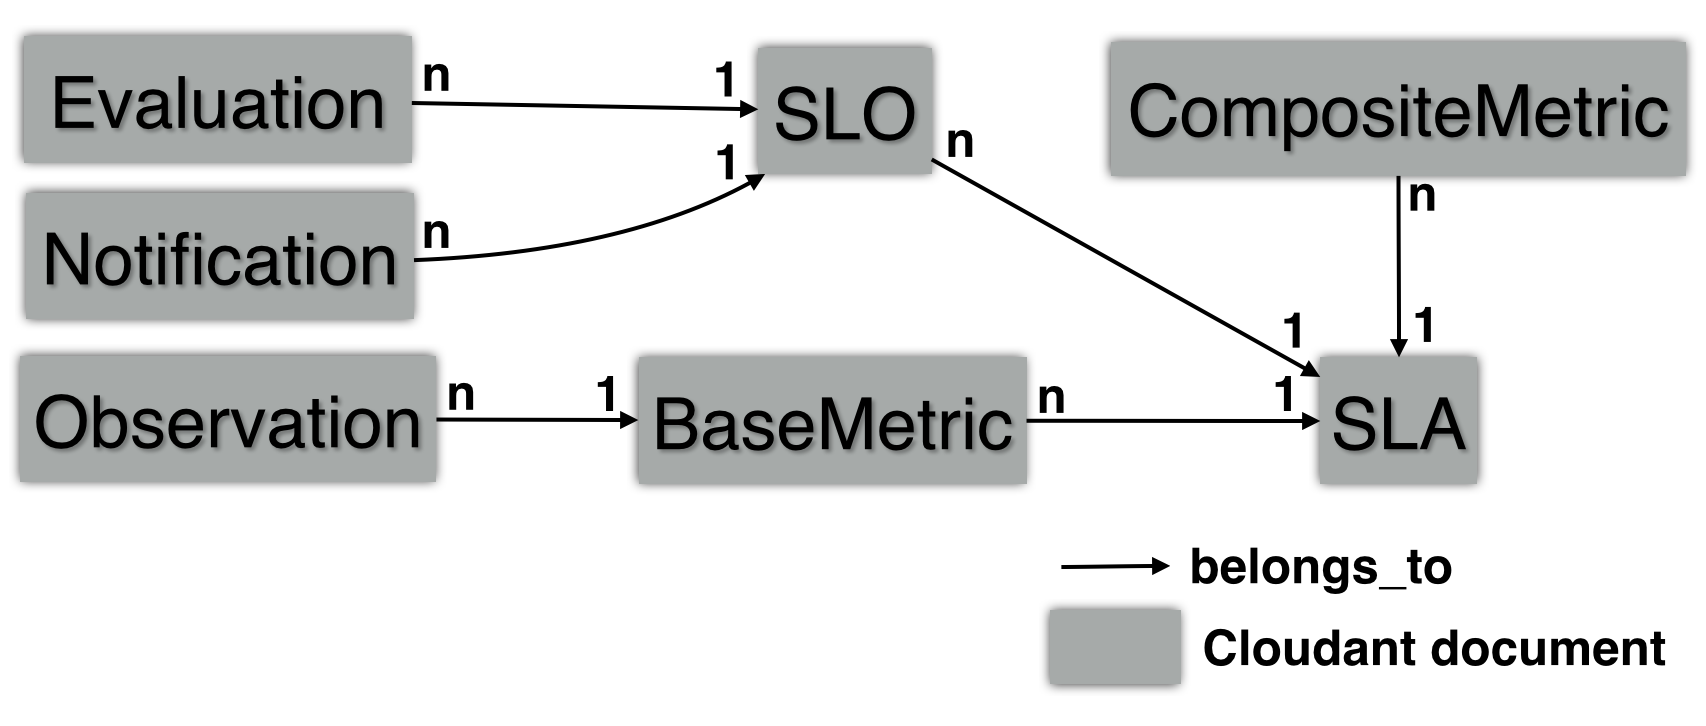
\includegraphics[width=0.8\textwidth]{pics/schema}
\caption{\label{rslaobject} rSLA Cloudant object associations}
\end{figure}

Processing, at the current implementation state, refers to compositions of service value sets for the creation of new rSLA objects.

timeseries: ready to use functions
\subsection{scheduling}\label{schedule}
The rSLA BaseMetric class provides methods for configuring a base metric object with one or more schedules.
\subsection{service level evaluation}

\subsection{notification reports}
can also be alerts
rSLA needs a source for monitoring data and a tool for reporting.